The properties of various moir\'e superstructure are well described in literature and Hermann gives a comprehensive overview in his paper \cite{hermann_periodic_2012}. One can conclude the following:

\begin{wrapfigure}{l}{4cm} \centering
	\subfigure[Isotropically scaled and aligned overlayer (gr/Pt(111): $p = 0.89$)]{
		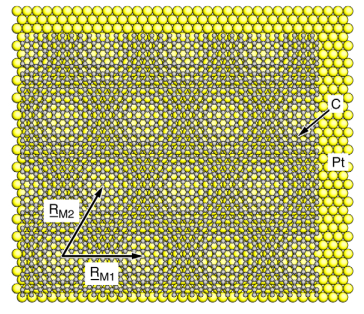
\includegraphics[width=0.25\textwidth]{./images/moire-scaled}%
		\label{fig:moire-pattern-scaled}
	}
	\subfigure[Isotropically scaled overlayer with rotation of \SI{5.4}{\degree} (gr/\textit{h}-BN: $p = 0.98$)]{
		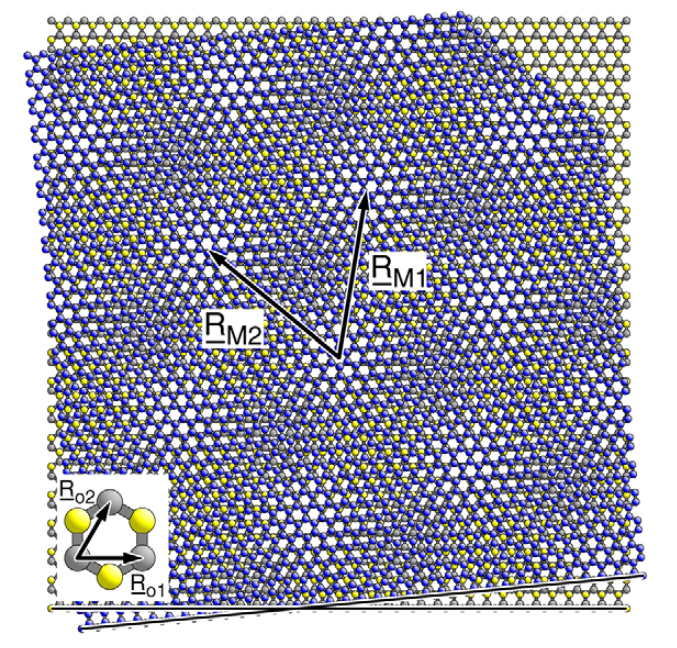
\includegraphics[width=0.25\textwidth]{./images/moire-scaled-rotated}%
		\label{fig:moire-pattern-scaled-rotated}
	}
	%	\subfigure[Isotropically scaled, alligned layer overgrowing a step edge (gr/Ir(111): $p = 0.91$)]{
	%		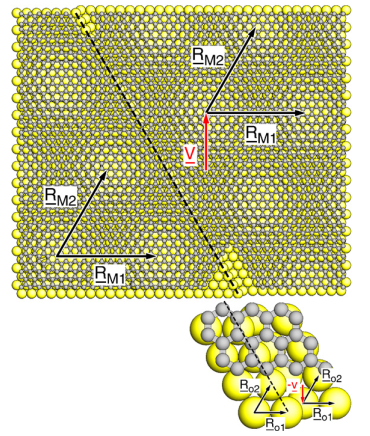
\includegraphics[width=0.25\textwidth]{./images/moire-scaled-step-edge}%
	%		\label{fig:moire-pattern-scaled-step-edge}
	%	}
	\caption{Adopted from \cite{hermann_periodic_2012}}
	\label{fig:moire-pattern}
\end{wrapfigure}

If lattice constants are equal like in the case of a graphene bilayer, the needed lattice mismatch occurs due to a rotation of the two layers. A moir\'e is always present if an over layer shows a lattice mismatch with respect to the substrate. 

For \textbf{isotropically scaled over layers} (refer to figure \ref{fig:moire-pattern-scaled}) one can calculate the scaling factor $$p=\frac{R^{'}_{O1}}{R_{O1}}$$ which gives the size of the over layer lattice in units of the substrate lattice. The moir\'e pattern shows the same Bravais lattice type than the substrate\cite[10]{hermann_periodic_2012}. If moir\'e and ad layer lattice are aligned ($\alpha=0$\textdegree) the direction of moir\'e and substrate is aligned. If the over layer is isotropically scaled and not rotated, the period of the moir\'e calculates to $$a_{moir\'e}=\underbrace{\frac{p}{|p-1|}}_{\kappa}a_{substrate}$$. With $a_{moir\'e}$ and $a_{substrate}$ are experimentally available, the ad layer lattice can be calculated with high precision (usually one order of magnitude more accurate than direction measurement of its period).

For a \textbf{scaled and rotated over layer} (figure \ref{fig:moire-pattern-scaled-rotated}, the angle between substrate and moir\'e ($\gamma$[rad]) scales with the angle between over layer and substrate ($\alpha$[rad]) as $\alpha=(1-p)\gamma$.

For rotated and isotropically scaled over layers, one can determine the $\alpha$ and $p$ from experimental observables $\gamma$(moir\'e angle to substrate) and $\kappa$(scaling factor) through relations $ \tan(\alpha)=\frac{sin(\gamma)}{cos(\gamma)+\kappa}\qquad p=\frac{\kappa}{\sqrt{1+\kappa^2+2\kappa cos(\gamma)}}$

When a scaled over layers over grows a step edge, the moir\'e pattern is altered. While period and orientation remain the same, a lateral shift in the superstructure is observed that interrupts the regular pattern and shifts subsequent moir\'e features by a vector $\vec{V}$.

\begin{figure} \centering
	\subfigure[DFT simulation of \textit{h}-BN on Ir(111). The moir\'e unit cell as well as regions where B and N atoms occupy high-symmetry positions w.r.t. the Ir lattice are indicated. The change in adsorption height is caused by the changing registry of substrate (Ir) and ad layer atoms (B,N).  Adopted from \cite{schulz_epitaxial_2014}]{
		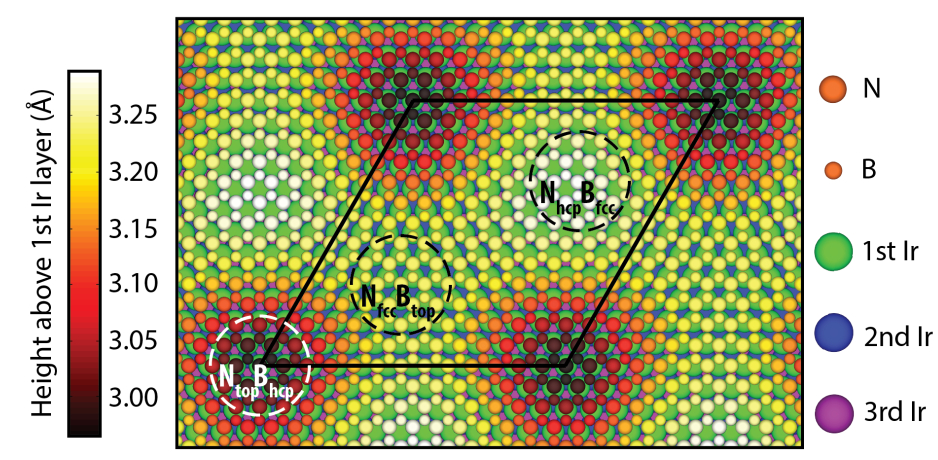
\includegraphics[width=0.5\textwidth]{./images/h-BN_Ir-moire}%
		\label{fig:h-BN-Ir-moire-DFT}
	} \qquad
	\subfigure[STM image of h-BN grown with CVD on Ir(111)]{
		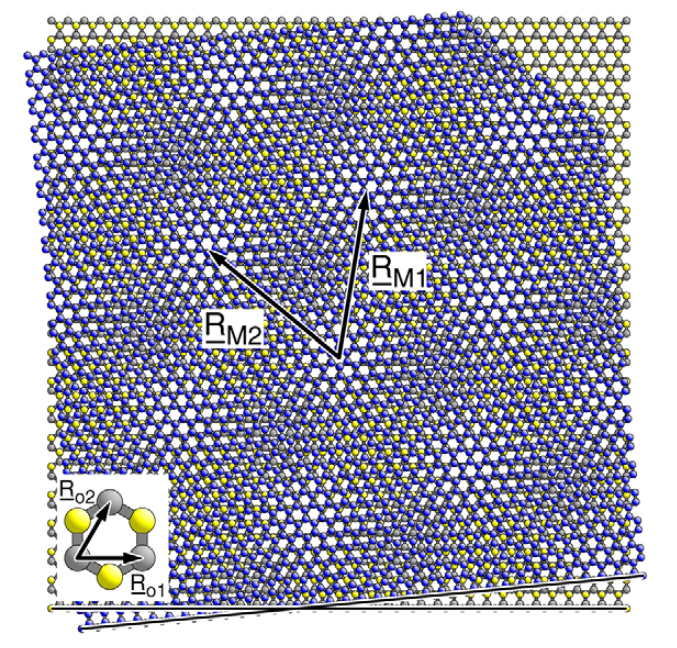
\includegraphics[width=0.25\textwidth]{./images/moire-scaled-rotated}%
		\label{fig:h-BN-Ir-moire-STM}
	}
	\caption{DTF calculation and STM images of \textit{h}-BN/Ir(111). While being aligned, a lattice mismatch creates a moir\'e  superstructure. It is well visible in adsorption height calculations \ref{fig:h-BN-Ir-moire-DFT} and as apparent height differences in STM images \ref{fig:h-BN-Ir-moire-STM}.}
	\label{fig:moire-DFT-TSM}
\end{figure}


\paragraph{Periodic change in work function}
A direct result of the lattice mismatch between ad layer and substrate is the alternating registry of ad layer atoms and substrate. In the following some resulting effects are discussed - namely the change in work function and its effects on the electronic structure of adsorbates.